% acm paper format
% \documentclass[sigconf]{acmart}
%
% \usepackage{booktabs}
%
% \setcopyright{rightsretained}
%
% DOI
% \acmDOI{10.475/123_4}
%
% ISBN
% \acmISBN{123-4567-24-567/08/06}
%
%Conference
% \acmConference[PODC'17]{ACM Symposium on Principles of Distributed Computing}{July 2017}{Washington, D.C., USA}
% \acmYear{2017}
% \copyrightyear{2017}
% end acm paper format

% article paper format
\documentclass[11pt,letterpaper]{article}

\usepackage{graphicx}
\usepackage[margin=1in]{geometry}
\usepackage{authblk}
\usepackage{amssymb}
% end article paper format

\title{Brief Announcement: Hierarchical Consensus for Scalable Strong Consistency}
\date{}

% acm author format
% \author{Benjamin Bengfort}
% \affiliation{%
%   \institution{University of Maryland}
%   \streetaddress{}
%   \city{College Park}
%   \state{Maryland}
%   \postcode{20742}
% }
% \email{bengfort@cs.umd.edu}
%
% \author{Pete Keleher}
% \affiliation{%
%   \institution{University of Maryland}
%   \streetaddress{}
%   \city{College Park}
%   \state{Maryland}
%   \postcode{20742}
% }
% \email{keleher@cs.umd.edu}
% end acm author format

% regular author format
\author[ ]{Benjamin Bengfort}
\author[ ]{Pete Keleher}
\affil[ ]{University of Maryland}
\affil[ ]{\textit{\{bengfort,keleher\}@cs.umd.edu}}
% end regular author format


\begin{document}

% \begin{abstract}
% Distributed consensus algorithms are the primary mechanism of implementing strong
% consistency in geo-replicated data stores.
% Consistency is guaranteed by the explicit sequential ordering of accesses or locks and
% leader based consensus protocols minimize the number of messages required to apply a
% command without conflict detection in a fault-tolerant manner.
% However, distributed consensus algorithms must reject inconsistent updates to the system
% and as a result do not provide high availability or throughput.
% In this paper we describe \emph{Hierarchical Consensus}, a new decentralized consensus
% protocol which distributes consensus decisions to multiple tiers of consensus groups
% according to shared accesses so as to maintain implicit dependencies.
% Hierarchical Consensus is unique in that it can efficiently guarantee the strict total
% ordering on replicated logs in the wider area even in the presence of partitions and
% varying connectivity. We will show its correctness and describe an experimental
% methodology that we will use to demonstrate durable, highly-available, and strongly
% consistent accesses in systems that scale from small to large networks.
% \end{abstract}

\maketitle

\section{Introduction}

Strong consistency in a geo-replicated distributed data store requires a fault-tolerant
mechanism that maintains consistency during node failure and communication partitions.
Distributed consensus protocols inspired by Paxos \cite{lamport_paxos_2001} have been
widely adopted to coordinate consistency, however, because of increased communication
they cannot scale to arbitrary system sizes\cite{2016arXiv160806696H}.
Several recent algorithms have attempted to address the scaling limitations of consensus
and take two general forms --- leader election and conflict detection.

Leader-oriented consensus such as MultiPaxos \cite{lamport_paxos_2001} and Raft
\cite{ongaro_search_2014} minimize the number of required communication phases by
nominating a dedicated proposer.
Less communication means better throughput, and fault-tolerance is achieved through node
failure detection such as a heartbeat and a new leader is elected to minimize downtime.
Leader-oriented approaches introduce two new problems, however: \emph{load} and
\emph{distance}.
Because the leader will necessarily do more work and handle more communication than other
nodes, it must have sufficient resources to handle the workload; moreover, since any node
can be elected leader, all nodes must have sufficient resources to handle the workload.
This introduces scaling problems in two dimensions: adding nodes means more communication,
increasing the minimum resource requirements for all nodes in the system.
In geo-replicated systems, bandwidth and latency are highly variable therefore the
election of a leader in a specific location means that consensus is bound by the slowest
connection, making the consensus algorithm sensitive to distance.
Although recent approaches such as S-Paxos \cite{biely_s-paxos:_2012} and Mencius
\cite{mao_mencius:_2008} add load balancing to leader-oriented mechanisms, they cannot
solve the distance problem.

Conflict detection approaches such as EPaxos \cite{moraru_there_2013} and MDCC
\cite{kraska_mdcc:_2013} are optimistic that most consensus decisions are consistent.
They propose ``fast'' and ``slow'' consensus paths, such that a subset of close nodes can
quickly reach consensus but add dependency information to detect conflicts when commands
are applied.
If a conflict is detected, then decision must traverse the ``slow'' path to ensure
correctness.
Conflict detection does not have a distance problem, as nodes can select close neighbors,
however this method does not guarantee dissemination of the command, which can require
large amounts of dependency resolution.
As the network scales, dependency graphs tend to increase in both size and complexity,
increasing the load on the system.

In practice systems do not implement global consensus, but instead apply multiple
consensus groups to coordinate specific objects or tablets.
This keeps quorum sizes small, allocating just enough nodes to a quorum to maintain a
minimum level of fault tolerance.
However, in so doing, an object can only be consistent with respect to its own updates
and the system loses information about dependencies.
Moreover, there is no coordination between consensus groups, a single node can
participate in multiple per-object consensus groups, which does not eliminate node and
distance problems.

% Probably need to hoist this paragraph up, and remove some of the problem statement
% stuff in the paras above.

In this paper we introduce \emph{Hierarchical Consensus}, an approach to generalize
consensus that allows us to scale groups beyond a handful of nodes, across wide areas.
Hierarchical Consensus (HC) increases the availability of consensus groups by
partitioning the decision space and nominating a leader for each partition.
Partitions eliminate distance by allowing decisions to be co-located with replicas that
are responding to accesses. Hierarchical consensus is flexible locally, but provides
strong global system guarantees.

\section{Consistency and Consensus}

We consider a set of processes $P = \{p_i\}_{i=1}^n$ which are connected via an asynchronous network, whose connections are highly variable.
The variability of a communication link between $p_i$ and $p_j$ is modulated by the
physical distance of the link across the geographic wide area.
Each process maintains the state of a set of objects, $O = \{o_i^v\}_{i=1}^m$, which are
accessed singly or in groups at a given process and whose state is represented by a monotonically increasing version number, $v$. There are two primary types of accesses, \texttt{read}, which returns the current versions of the accessed objects, and \texttt{update}, which increments the versions of the accessed objects.

Strong consistency across all process requires a global ordering of accesses. The strongest consistency, \emph{linearizablity}, requires the ordering of both \texttt{read} and \texttt{update} operations. \emph{Sequential consistency} allows for concurrent accesses so long as there is some globally defined ordering, which is specified by the \texttt{happens-before} relation ($\rightarrow$). Sequential consistency therefore only considers \texttt{update} operations but specifies an ordering of updates, maintaining a sequence $o_i^w \rightarrow o_i^{w+1} \rightarrow o_j^x$ and so forth. Objects that are accessed together (by the same process and within a defined window of time) are implicitly dependent on each other, requiring their relative access order to be strictly defined. Objects that are not implicitly dependent on each other, e.g. accessed by separate processes, do not require a strict ordering and can instead be arbitrarily ordered by process id.

Distributed consensus protocols implement strong consistency by maintaining an ordered log of accesses (commands). Once a leader has been elected (a dedicated proposer), accesses are forwarded to the leader who, after checking application-specific invariants, broadcasts a request to other nodes to append the access to their log. A decision is reached when a majority of the quorum accept the append, at which point the leader sends a commit message. Fault-tolerance is observed by nodes that fall behind by replaying the log of committed accesses until they are up to date. Correctness is maintained by observing communications failure from the leader and electing a new leader.

\section{Hierarchical Consensus}

Hierarchical consensus conducts coordination decisions as a tier of quorums such that
parent quorums manage the decision space and leaf quorums manage access ordering.
Hierarchical consensus considers the decision space as subsets of the object set, and
subquorums are defined by a time-annotated disjoint subset of the objects they maintain,
$Q_{i,e} \subset O$.
The set of subquorums, $Q$ is not a partition of $O$, but only represents the set of
objects that are being accessed at time $e$.

% The E_i notation doesn't really match with the Q_{i,e} notation, not sure what to do.

The hierarchical consensus algorithm starts with a root quorum whose main
responsibilities are i) the mapping of objects to subquorums and ii) the mapping of
replicas to subquorums.
Each instance of such a map defines a distinct \emph{epoch}, $E$, a monotonically
increasing representation of the term of $Q_e$.
Decisions that require a modification of the decision space or changes the mapping of
objects or replicas to subquorums requires a new \emph{epoch}. The fundamental
relationship between epochs is as follows: any access that happens in epoch
$E_i \rightarrow E_{i+1}$. Alternatively, any access in epoch $E_{i+1}$
\emph{depends on} all accesses in epoch $E_i$.
Accesses in different subquorums but in the same epoch happen concurrently from the global
perspective, though accesses in a specific subquorm are totally ordered locally.

\subsection{Operation}

The parent consensus group must coordinate all decision space changes.
Consider the simple example of the transfer of object responsibility from one subquorum
to another:

% Pete: I'm not a fan of this notation, was just following from what I had above. I think
% we could probably go back to the ABC --> ABGH notation.
\begin{quote}
\small
   $Q_1: \{o_a,o_b,o_c\} \rightarrowtail \{o_a,o_b,o_g,o_h\}$\\
   $Q_2: \{o_d,o_e,o_f,o_g,o_h\} \rightarrowtail \{o_c,o_d,o_e,o_f\}$
\end{quote}

Each of the two subquorums, $Q_1$ and $Q_2$, wants to give up a portion of its
existing decision space, and to add objects currently mapped to another subquorum.
In order to reallocate the subquorums, a two phase consensus decision is required.
Both subquorum leaders make change requests to the leader of the parent quorum, who may
aggregate several namespace changes into a single one.
While the parent quorum gets consensus to make the epoch change, subquorums can continue
operating on their own decision space.
Once the parent quorum updates the epoch, it communicates the change to all affected
subquorums.
Each such subquorum then increments its epoch and acknowledges its change to the parent
quorum.
At this point, the subquorum can operate on the portion of the decision space it owned
before, \emph{but not the objects that are being added}.
Once the parent quorum gets confirmations of epoch update from all subquorums, it notifies
the subquorums that they can begin operating on the complete subset of objects from the
new epoch.

All accesses to an object must be forwarded to the leader of the subquorum that contains
the object.
Objects that are accessed together or who have application-specific, explicit
dependencies (such as the set of objects included in a transaction) must be part of the
same subquorum so that local accesses are totally ordered.
Dependent objects that are not part of the same subquorum require either a change in
epoch or a mechanism to facilitate \emph{remote accesses}, which we will discuss in a
following section.

\subsection{Epochs and Ordering}

Hierarchical consensus requires all accesses in all subquorums to be at least
sequentially consistent.
Local sequential consistency is guaranteed by serializing all accesses through a leader.
Global sequential consistency is guaranteed by serializing epochs at the parent quorum.

Let \emph{interval} $i_n$ be the ordered set of accesses of the replicas in subquorum
$Q_i$ during epoch $E_n$.
We enforce sequentially consistent ordering of all accesses in the entire system by
ensuring that there must exist a total ordering of the intervals that produces the correct
access results.
Access results should be equivalent to any interval ordering
such that all intervals in $E_n$ occur before intervals in $E_{n+1}$ (our ``interval
ordering'' invariant).
This is because there is no cross-traffic between any $Q_i$ and $Q_j$, and therefore
ordering interval $i_n$ before $j_n$ is exactly the same as ordering interval $j_n$
before $i_n$, for any $i$, $j$, and $n$.

The internal invariant requires $\forall_{x,y} : Q_{x,i} \rightarrow Q_{y,i+1}$.
Ordering all accesses according to log order and interval order satisfies both the
internal invariant and sequential consistency while still allowing subquorums to operate
independently within epochs.
Given $Q_i$ and $Q_j$ within epochs $E_1$ and $E_2$, one possible interval order is
$Q_{i,1} \rightarrow Q_{j,1} \rightarrow Q_{i,2} \rightarrow Q_{j,2}$.

\subsubsection{Remote Accesses}

By default we assume that the set of replicas \emph{assigned} to subquorums are also
disjoint, and that all accesses through a replica of a given subquorum are mapped to the
local decision space.
This is often reasonable.
However, if an object is assigned to a decision space and another subquorum wishes to
access it, the system must either disallow the access (our default approach) or take
explicit notice that a dependency has been created between the subquorums.

The latter approach requires a serialization of all accesses currently within the remote
quorum with respect to all accesses prior to the remote access in the local quorum.
Assume a read access from $Q_k$ to $Q_i$ in epoch $e$; at the time of the read all
accesses in $Q_i$ must $\rightarrow$ all accesses following the read.
We accommodate this requirement by using the read endpoints to break interval $i_e$ into
$i_{e.1}$ and $i_{e.2}$ at the point $Q_i$ receives the remote access, and interval $k_e$
into $k_{e.1}$ and $k_{e.2}$ at the point $Q_k$ receives a response.
Our results are consistent with total interval ordering by incorporating $Q_{i.1}
\rightarrow Q_{i.2}$.
Remote accesses are expensive and the runtime system must weight the cost of repeated
remote accesses against the cost of an epoch change.

\subsubsection{Fuzzy Epochs}

Only the subquorums that are involved in the  decision space changes need be notified and
involved in the epoch change coordinated by parent epochs.
Other subquorums can update their epoch number at no cost when they see the new epoch
number from remote requests from other subquorums, or when they are notified by their
parent quorum.
In this way, non-responding subquorums do not block decision space changes for other
quorums.
Because the subquorum is left behind in the previous epoch, all writes in that subquorum
will be ordered before writes in the next epoch.
However, because no writes in the next epoch depend on these writes safety is still
guaranteed.

This means that subquorums can have ``fuzzy epochs'', wherein some subquorums are behind
others.
Fuzzy epochs provide the flexibility needed to accommodate subquorums that may not be
ready to move to a new epoch eliminate because application semantics (still accessing the
same objects), or network conditions (communication failure).

\begin{figure}[t]
    \centering
    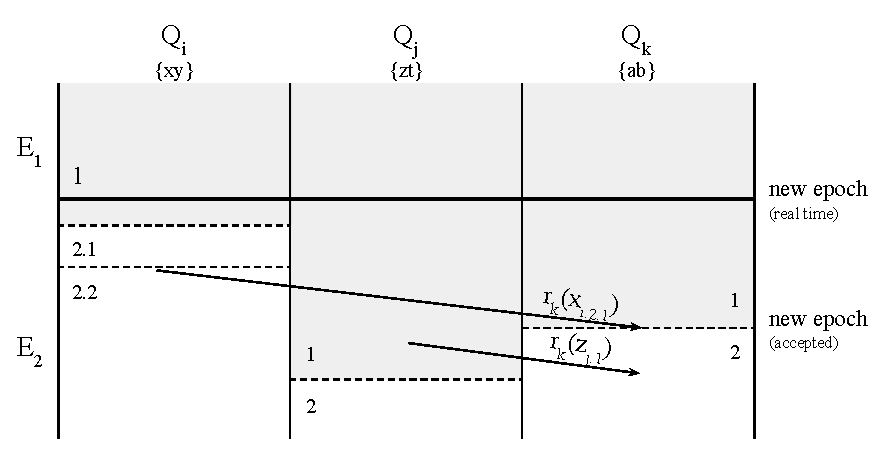
\includegraphics[height=0.2\textheight]{figures/fuzzy}
    \caption{The gray region shows the ``fuzzy'' boundary between epochs $E_1$ and $E_2$.}
    \label{fig:fuzzy}
\end{figure}

Figure \ref{fig:fuzzy} shows three subquorums.
The gray boundary delineates the border between epochs $E_1$ and $E_2$ -- it is fuzzy
because not all subquorums move to epoch $E_2$ at the same time.
The first read access, $r_k(x_{2.1})$, reads the value of object $x$ from $Q_i$ into
$Q_k$.
However, $Q_i$ is in $E_2$ when it services the read, while $Q_k$ is still in $E_1$ when
the value is returned.
If we follow the remote access approach, we can divide interval $i_2$ into $i_{2.1}$ and
$i_{2.2}$, and $k_1$ into $k_{1.1}$ and $k_{1.2}$.
We must also insure accesses are consistent with the interval ordering invariant, but
this is not maintained because of the new dependency $i_{2.1} \rightarrow k_{1.1}$.
Therefore, data coming from an interval in $E_n$ requires the receiver to also transition
to $E_n$. This allows us to instead break our interval $i$ as before and maintain the
ordering $i_{2.1} \rightarrow k_2$.

\section{Correctness}

% not feeling good about this section ... probably just remove it?

We assert that consensus at the leaf nodes is correct and safe because decisions are
implemented using well-known leader-oriented consensus approaches.
Because decision allocation occurs on accesses and is defined by a fixed period of time,
we propose to show correctness through \emph{eventual quiescence}.
Quiescence refers to the property that subquorums disband and return object ownership
back to the parent quorum if activity ceases.
Because all changes to the decision space require incrementing the epoch, if only the
root quorum exists, the epoch is closed (e.g. no accesses will be applied to a log with
that epoch).

The primary case to consider is an unsafe append to the access log: $Q_{i,e}$
appends object $o_a^{v+1}$ while $Q_{j,e+1}$ appends object $o_a^v$ (incorrectly
specifying that $o_a^{v+1} \rightarrow o_a^v$).
It is the parent quorum's responsibility to ensure that $Q_{j,e+1}$ does not start
operating until it has received confirmation from $Q_{i,e}$ that it has terminated.
If the parent quorum does not receive a message from $Q_{i,e}$, it can enforce quiescence
-- closing epoch $e$, and then return control to $Q_{j,e+1}$. This causes all accesses in
$Q_{i,e}$ to be dropped when it communicates with the leader.

% \section{Experimental Design}
%
% We propose to implement a distributed file system called FluidFS to more completely explore
% the use of hierarchical consensus in supporting file systems.
% FluidFS, implemented in the Go programming language, will allow us to quantitatively
% describe real-world environments and usage and to show how our proposed consistency
% model is experienced by users.
%
% FluidFS will provide \emph{close-to-open consistency} (CTO), meaning that a file
% open, which implies a full-file read, is guaranteed to see the data written by the ``most recent'' close of
% that file.
% Therefore file opens and closes must be totally ordered, and map
% easily onto operations in a replicated log.
% The canonical use of CTO is a single-server case, where a total
% ordering of file open and closes is just the ordering that the opens
% and closes arrive at the server.
% The distributed case assumed by this work is much more demanding because
% opens and closes are distributed across servers throughout the system.
%
% We leverage hierarchical consistency to build a distributed set of sequentially-consistent logs
% that guarantee a total ordering over all file accesses.
% The result is a similar user experience to having the user/client co-located with a single
% server, while the user migrates around the system, using different devices, possibly
% collaborating with other users, and tolerating network vagaries, partitions, and failures.
%
% Note that FluidFS, like many modern file systems,
% decouples metadata file
% data storage~\emph{recipes}
% Metadata includes an ordered list of \emph{blobs}, which are opaque binary chunks.
% When a file is closed after editing, the data associated with the file is chunked into a
% series of variable-length blobs, identified by a hashing function applied to
% the data.
% The version created by the write access to the file specifies the blobs and their ordering
% that make up the file.
% Since blobs are effectively immutable, or tamper-evident, (blobs are named by hashes of
% their contents), we assert that consistent metadata replication can be decoupled from blob
% replication.
% Accesses to file system metadata becomes the operations or entries in the replicated logs.
% Metadata is therefore replicated through the system, allowing any file
% system client to have a complete view of the file system namespace.

\section{Discussion}

Hierarchical consensus flexibly allocates subquorums to dynamic object groupings.
Multiple subquorums means both more leaders and less global communication, reducing the
resource requirements for most nodes, preventing bottlenecks, and increasing throughput.
Consensus decisions can also be localized to where the accesses are occurring,
minimizing both distance and the effect of wide area network variability.
Finally, hierarchical consensus does not arbitrarily assign consensus decisions to single
objects or unrelated groups of objects, but to objects that are implicitly dependent on
each other because of their associated accesses.

An open question for our research is how to automatically allocate the namespace such that
leadership of a subset of the namespace is local to the accesses and that members of the
quorum are distributed to provide wide area durability and availability.
To explore this question as well as empirically show the scalability of hierarchical
consensus, we are currently implementing a distributed file system called FluidFS.
FluidFS will allow us to quantitatively describe real world environments and usage and
to demonstrate how our proposed consistency model is experienced by users.

\bibliographystyle{plain}
\bibliography{paper}

\end{document}
